 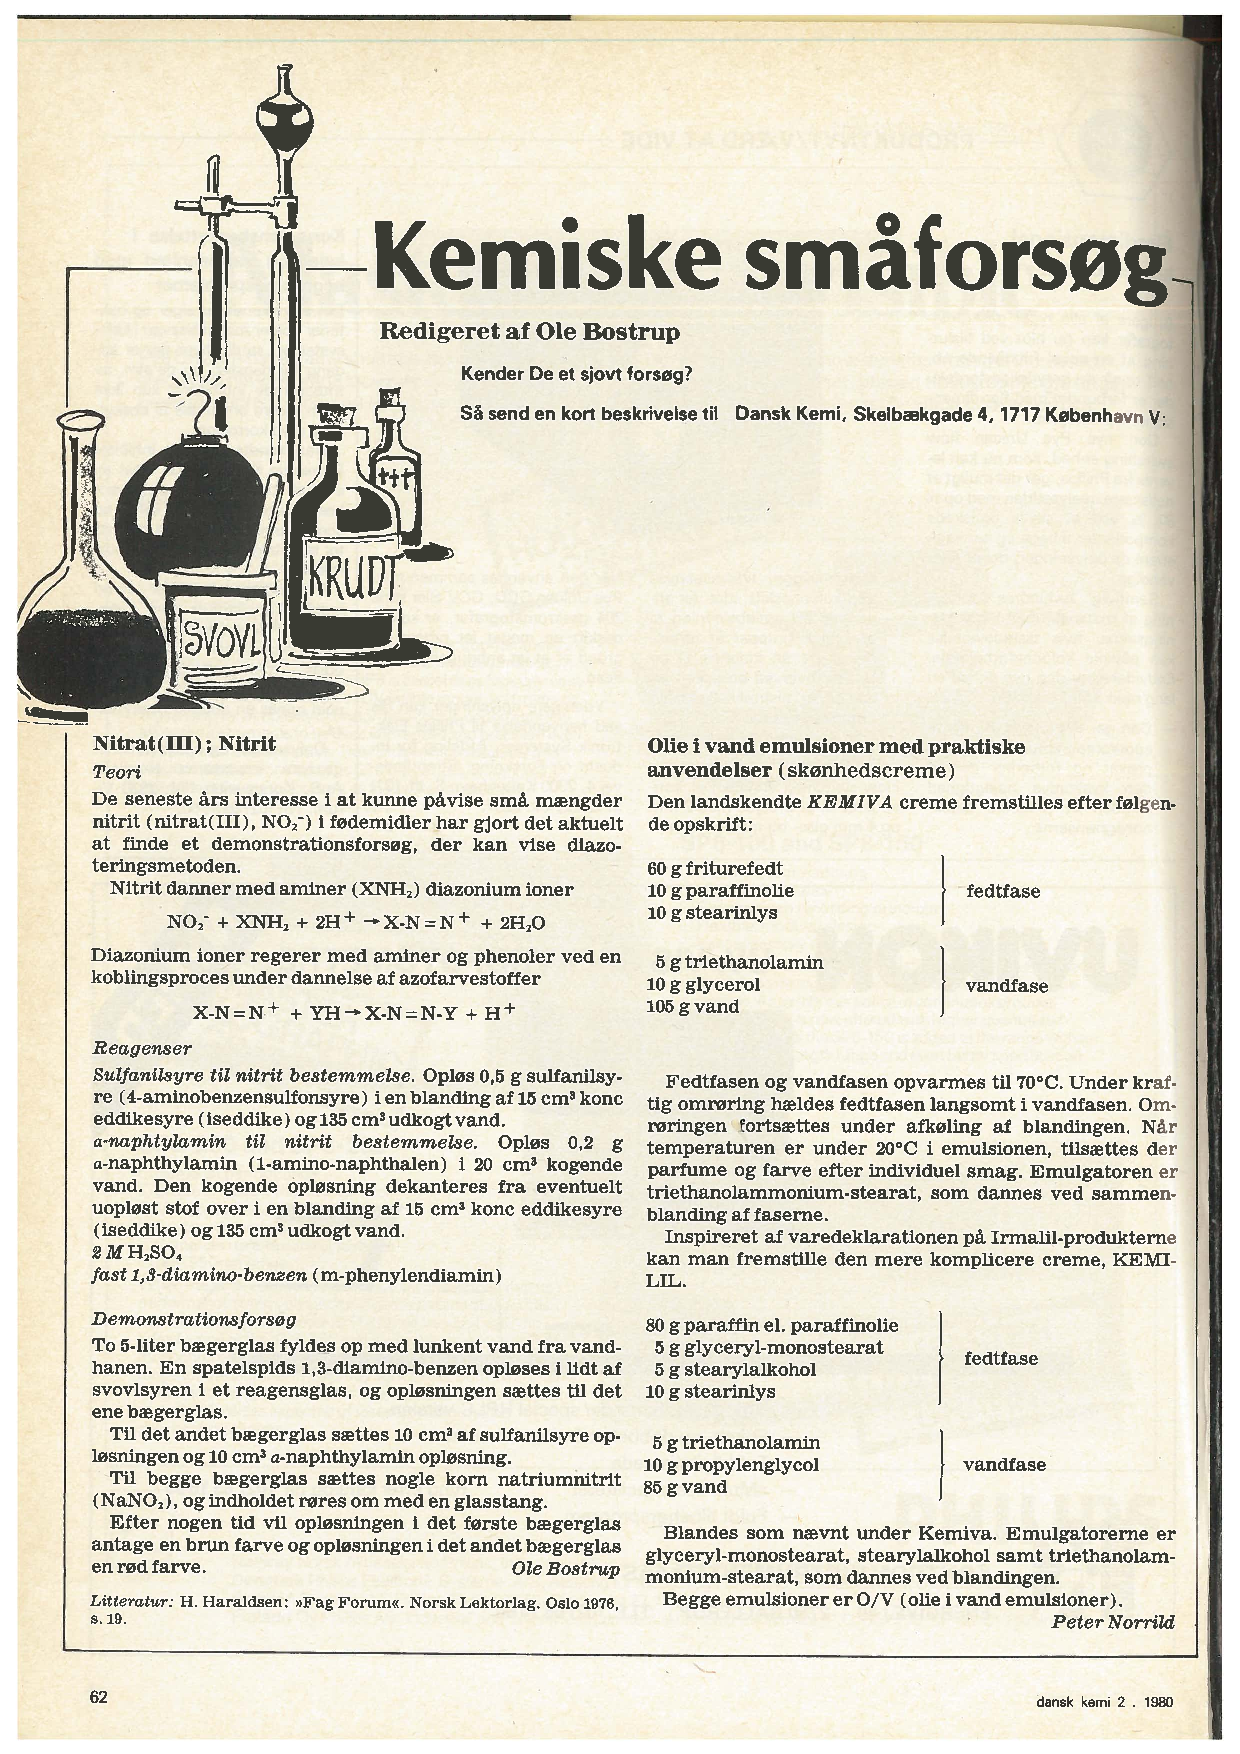
\includepdf[pages=-]{pdfs/1980-61-2-62.pdf}

\emne{Nitrat (III); Nitrit}
dansk kemi vol 61 iss 2 p 62

Teori

De seneste års interesse i at kunne påvise små mængder nitrit (nitrat(III), NO2-) i fødemidler har gjort det aktuelt at finde et
demonstationsforsøg, der kan vise diazoteringsmetoden.
Nitrit danner med aminer (XNH2) diazonium ioner

\ch{NO2- + X NH2 + 2 H+ -> X-N=N+ + 2 H2O}

Diazonium ioner regerer med aminer og phenoler ved en koblingsproces
under dannelse af azofarvestoffer
\ch{X-N=N+ + YH -> X-N=N-Y + H+}

Reagenser
Sulfanilsyre til nitrit bestemmelse. Opløs 0,5 g sulfanilsyre
(4-aminobenzensulfonsyre) i en blanding af 15 cm3 konc eddikesyre
(iseddike) og 135 cm3 udkogt vand.
a-naphtylamin til nitrit bestemmelse. Opløs 0,2 g a-naphthylamin
(1-amino-naphthalen) i 20 cm3 kogende vand. Den kogende opløsning
dekanteres fra eventuelt uopløst stof oer i en blanding af 15 cm3
konc eddikesyre (iseddike) og 135 cm3 udkogt vand.
2 M H2SO4
fast 1,3-diamino-benzen (m-phenylendiamin)

Demonstrationsforsøg
To 5-liter bægerglas fyldes op med lunkent vand fra vandhanen.
En spatelspids 1,3-diamino-benzen opløses i lidt af svovlsyre i et
reagensglas, og opløsningen sættes til det ene bægerglas.
Til det andet bægerglas sættes 10 cm3 af sulfanilsyre opløsningen og
10 cm3 a-naphthylamin opløsning.
Til begge bægerglas sættes nogle korn natriumnitrit (NaNO2) og indholdet
røres om med en glasstang.
Efter nogen tid vil opløsningen i det første bægerglas antage en
brun farve og opløsningen i det andet bægerglas en rød farve.

Forfatter: Ole Bostrup.
Litteratur: H. Haraldsen: "Fag Forum". Norsk Lektorlag. Oslo 1976, s. 19.
